\documentclass[12pt]{article}
\usepackage[spanish,mexico]{babel}
	\selectlanguage{spanish}
\usepackage{graphicx}
\usepackage{amsmath}
\usepackage{wrapfig}
\usepackage{float}
\usepackage[utf8]{inputenc}

\usepackage{graphicx}
\graphicspath{{images/}}

\usepackage{vmargin}
\setmarginsrb{3 cm}{1.0 cm}{3 cm}{1.0 cm}{1 cm}{1.5 cm}{1 cm}{1.5 cm}
\usepackage{listings}
\usepackage[usenames,dvipsnames]{color}
	\definecolor{ocre}{RGB}{42,105,21}
	\definecolor{ocre2}{RGB}{47,109,130}
	\definecolor{gray2}{gray}{0.95}
	\lstset{
		language=Python,
		backgroundcolor=\color{gray2},
		basicstyle=\color{black}\small\ttfamily, 
		breakatwhitespace=false,         
		breaklines=true,                 
		captionpos=b,                    
		columns=flexible,
		commentstyle=\color{ocre2}\ttfamily, 
		deletekeywords={...},            
		escapeinside={\%*}{*)},          
		extendedchars=true,             
		frame=single,	                 
		keepspaces=true,                 
		keywordstyle=\color{blue}\bfseries,       
		otherkeywords={*,...},          
		numbers=left,                    
		numbersep=5pt,                   
		numberstyle=\tiny, 
		rulecolor=\color{black},         
		showspaces=false,                
		showstringspaces=false,          
		showtabs=false,                  
		stepnumber=1,                    
		stringstyle=\normalfont\color{ocre},     
		tabsize=2,	                     
		title=\lstname                  
		}

\title{Actividad 5: Movimiento armónico simple:\\ Péndulo}
\author{Martin Alejandro Paredes Sosa}
\date{Marzo, 2016}

\begin{document}
\maketitle

\section{Introducción}
La matemática de un péndulo simple es, en general, compleja. Hacer suposiciones que simplifican la descripción nos permite resolver analíticamente las ecuaciones de movimiento para las oscilaciones de ángulos pequeños.\\
El péndulo simple, es una idealización se un péndulo real, pero en un sistema aislado donde se asume:
\begin{itemize}
	\item La cuerda tiene una masa despreciable, es rígida y se mantiene tensa.
	\item El péndulo se maneja como una masa puntual.
	\item El movimiento es en dos dimensiones trazando un arco.
	\item No pierde energía por fricción o resistencia al aire.
	\item El campo gravitacional es uniforme.
	\item El soporte no se mueve.
\end{itemize}

La ecuación que nos permite encontrar el periodo cuando se utilizan ángulos pequeños es:
\begin{equation}\label{PeriodoP}
	T_o = 2\pi\sqrt{\frac{\ell}{g}}
\end{equation}
Mientras que para cualquier angulo es:
\begin{equation}\label{PeriodoG}
	T = 4\pi \int^{\theta_o}_0 \frac{1}{\sqrt{cos\theta-\cos\theta_o}}d\theta
\end{equation}
donde $g$ es la aceleración de la gravedad, $\ell$ es la longitud del péndulo y $\theta_o$ es la condición inicial \cite{PendWiki}.

\section{Función \emph{integrate.quad}}
Para poder resolver la integral que se tiene en la ecuacion \eqref{PeriodoG} se utilizaron herramientas computacionales. En nuestro caso, para resolverla se utiliza la función \emph{integrate.quad} de la librería \emph{scipy} de Python \cite{scipy}.

Esta función utiliza los siguientes parámetros:
\begin{itemize}
	\item func:\textit{function}. Es la función definida anteriormente para integrar.
	\item a: \textit{float}. Limite inferior de integración
	\item b: \textit{float}. Limite superior de integración
	\item args:\textit{tuple, opcional}. Argumentos extra para la función.
\end{itemize}
%============================================================================================================
%\pagebreak
%============================================================================================================
\section{Ejercicio y Resultados}
Esta actividad consistió en realizar un código en python que nos permitiera encontrar el periodo de un péndulo para ángulos arbitrarios. Se hizo uso de la librería \emph{scipy.integrate} haciendo uso de la función \textit{quad}. Una vez que se tenia el periodo se gráfico el error relativo $T/T_o$ y se demostró como es que diverge el periodo a medida que el angulo inicial tiende a $\pi$.\\

El siguiente código fue el que se utilizo:
\lstinputlisting[caption={Programa Periodo.py}]{Periodo.py}
%============================================================================================================
\pagebreak
%============================================================================================================
Las gráficas que resultaron son las siguientes:
\begin{figure}[H]
\centering
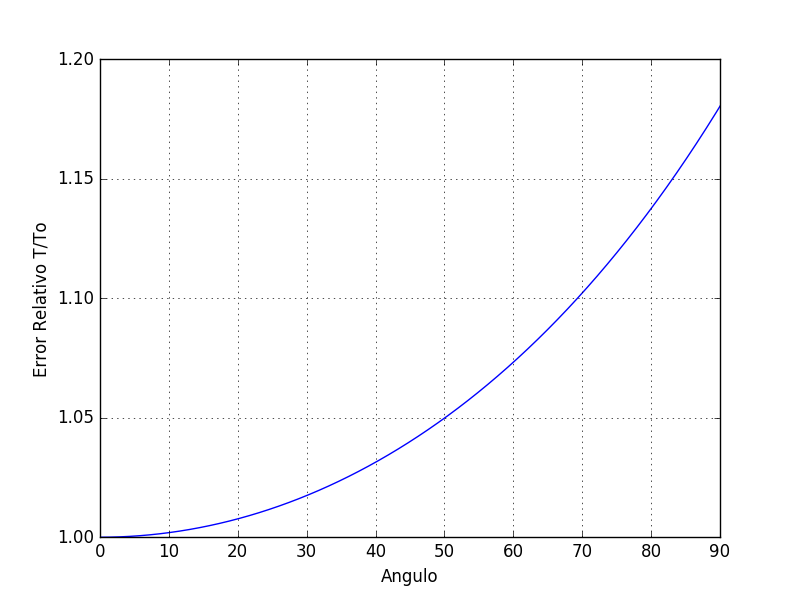
\includegraphics[width=15cm,height=8.5cm]{Error.png}
\caption{Angulo vs Error Relativo $T/T_o$}
\end{figure}
\begin{figure}[H]
\centering
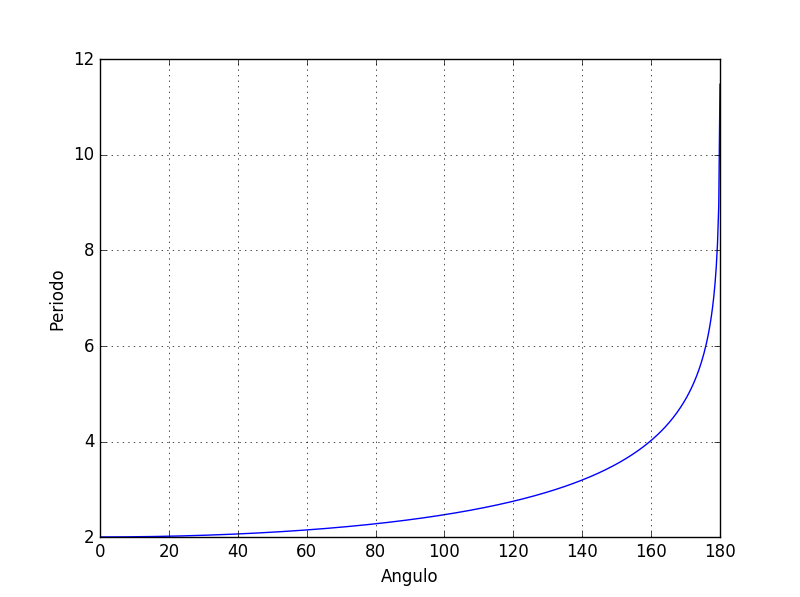
\includegraphics[width=15cm,height=8.5cm]{Divergencia.png}
\caption{Divergencia del Periodo}
\end{figure}
Como Se puede observar, error aumenta conforme el ángulo crece, ademas el periodo tiende a infinito cuando el ángulo tiende a $\pi$.

\begin{thebibliography}{3}

	\bibitem{PendWiki}
	Wikipedia,(2016)
	\emph{Pendulum (mathematics)}. Recuperado de\\
	https://en.wikipedia.org/wiki/Pendulum\_\%28mathematics\%29

	\bibitem{scipy}
	Scipy.org (2016)
	\emph{Integration and ODEs}. Recuperado de\\
	http://docs.scipy.org/doc/scipy/reference/generated/scipy.integrate.quad.html\\\#scipy.integrate.quad

	\bibitem{act}
	Lizárraga, C. (2016)
	\emph{Actividad 6 (2016-1)}. Recuperado de\\ 
	http://computacional1.pbworks.com/w/page/105233358/Actividad\%205\%20\\(2016-1)
	
\end{thebibliography}

\end{document}